% Latex template: mahmoud.s.fahmy@students.kasralainy.edu.eg
% For more details: https://www.sharelatex.com/learn/Beamer

\documentclass{beamer}					% Document class
\geometry{papersize={15cm,10cm}}

\setbeamertemplate{footline}[text line]{%
  \parbox{\linewidth}{\vspace*{-8pt}\hfill\hfill\insertpagenumber}}
\setbeamertemplate{navigation symbols}{}

\usepackage[english]{babel}				% Set language
\usepackage[utf8x]{inputenc}			% Set encoding

\mode<presentation>						% Set options
{
  \usetheme{default}					% Set theme
  \usecolortheme{default} 				% Set colors
  \usefonttheme{default}  				% Set font theme
  \setbeamertemplate{caption}[numbered]	% Set caption to be numbered
}

% Uncomment this to have the outline at the beginning of each section highlighted.
%\AtBeginSection[]
%{
%  \begin{frame}{Outline}
%    \tableofcontents[currentsection]
%  \end{frame}
\usepackage{graphicx}					% For including figures
\usepackage{booktabs}					% For table rules
\usepackage{hyperref}	
\usepackage{tikz-network}				% For cross-referencing
\usepackage[absolute,overlay]{textpos}
\usepackage{bm}
\usepackage[font=small,labelfont=bf]{caption}				% For cross-referencing
\usepackage{comment}

\title{Visualizing chromatin organization with time resolved single molecule localization microscopy}	% Presentation title
\author{Clayton W. Seitz}								% Presentation author
\date{\today}									% Today's date	

\setbeamertemplate{footline}{
    \hbox{%
    \begin{beamercolorbox}[wd=\paperwidth,ht=3ex,dp=1.5ex,leftskip=2ex,rightskip=2ex]{page footer}%
        \usebeamerfont{title in head/foot}%
        \insertshorttitle \hfill
            \insertsection \hfill
        \insertframenumber{} / \inserttotalframenumber
    \end{beamercolorbox}}%
}

\begin{document}

% Title page
% This page includes the informations defined earlier including title, author/s, affiliation/s and the date
\begin{frame}
  \titlepage
\end{frame}

\begin{frame}{Outline}
    \tableofcontents
\end{frame}



% The following is the most frequently used slide types in beamer
% The slide structure is as follows:
%
%\begin{frame}{<slide-title>}
%	<content>
%\end{frame}




\section{Single molecule localization microscopy}

\begin{frame}{Single molecule localization microscopy}
Localization: $\theta^{*} = \underset{\theta}{\mathrm{argmax}}\prod_{k}P(H_{k}|\theta)= \underset{\theta}{\mathrm{argmin}}-\sum_{k}\log P(H_{k}|\theta)$

\begin{textblock*}{8cm}(6.5cm,2.5cm)
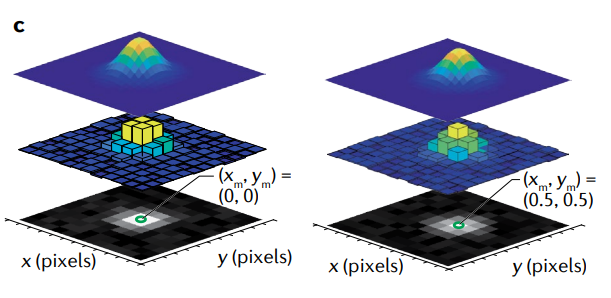
\includegraphics[width=\textwidth]{Model.png}
\end{textblock*}

\begin{textblock*}{2cm}(1cm,2.5cm)
\begin{align*}
\mu_{k} &= g_{k}\textcolor{red}{\eta} \textcolor{cyan}{N_{0}}\textcolor{blue}{\Delta}\int_{\mathrm{pixel}} G(x,y)dA\\
\\
\textcolor{red}{\eta} &- \mathrm{quantum\; efficiency}\\
\textcolor{cyan}{N_{0}} &- \mathrm{photon\; count}\\
\textcolor{blue}{\Delta} &- \mathrm{exposure\; time}
\end{align*}
\end{textblock*}

\vspace{2in}

\begin{itemize}
\item SMLM techniques are diffraction unlimited
\item Exposures are typically ten to hundreds of ms
\item SMLM techniques are suitable for \textbf{super-resolution} (SR) and \textbf{single molecule tracking} (SMT)
\end{itemize}

\end{frame}

\begin{frame}{A Poisson approximation at moderate SNR simplifies SMLM}

\begin{figure}
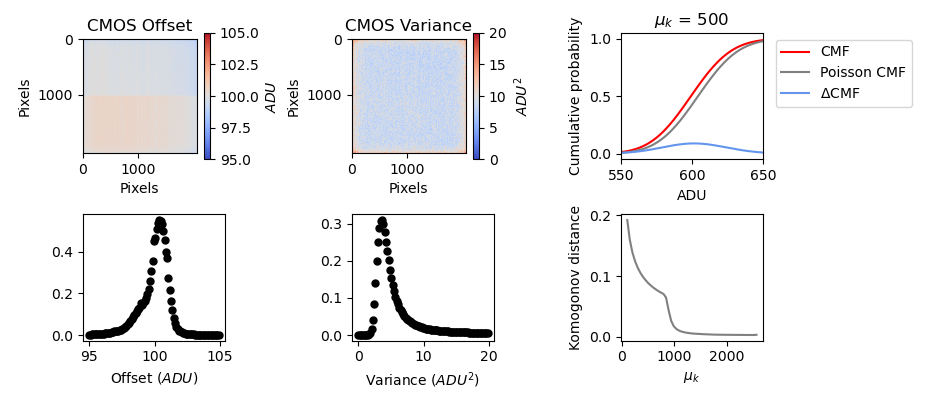
\includegraphics[width=13cm]{Noise.png}
\end{figure}

\begin{equation*}
P(H_{k}|\theta) = A\sum_{q=0}^{\infty} \frac{1}{q!}e^{-\mu_{k}}\mu_{k}^{q}\frac{1}{\sqrt{2\pi}\sigma_{k}}e^{-\frac{(H_{k}-g_{k}q-o_{k})}{2\sigma_{k}^{2}}}
\end{equation*}

$P(H_{k}|\theta)$ can be approximated as Poisson at high signal-to-noise ($\mathrm{SNR}$)
 
\end{frame}

\begin{frame}{Estimator precision in localization microscopy}
\begin{textblock*}{4cm}(1.0cm,1.0cm)
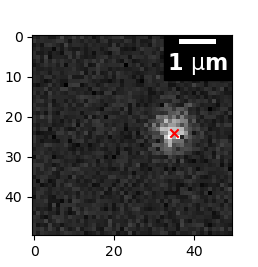
\includegraphics[width=4cm]{MCMC/Figure_1.png}
\end{textblock*}
\begin{textblock*}{4cm}(1.0cm,5cm)
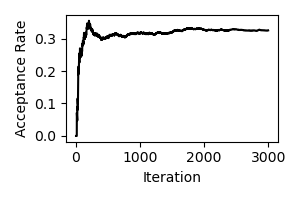
\includegraphics[width=4cm]{MCMC/Figure_2.png}
\end{textblock*}
\begin{textblock*}{9cm}(5cm,1.0cm)
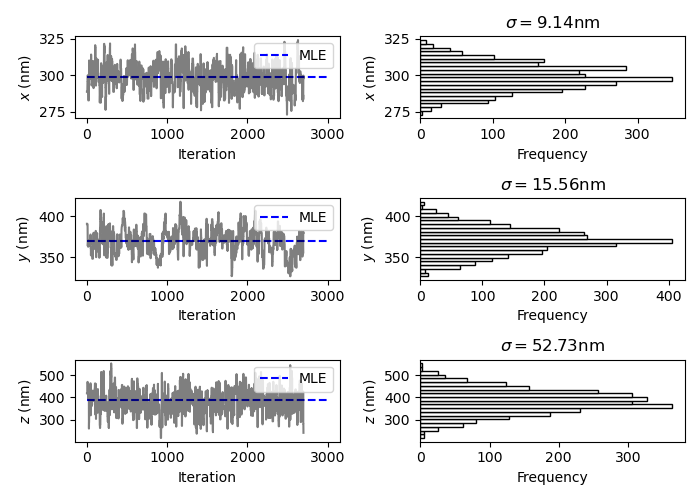
\includegraphics[width=9cm]{MCMC/Figure_3.png}
\end{textblock*}
\begin{textblock*}{13cm}(0.5cm,8cm)

\end{textblock*}
\end{frame}

\begin{frame}
\frametitle{Super resolution with photoswitching of rhodamines}

\begin{figure}
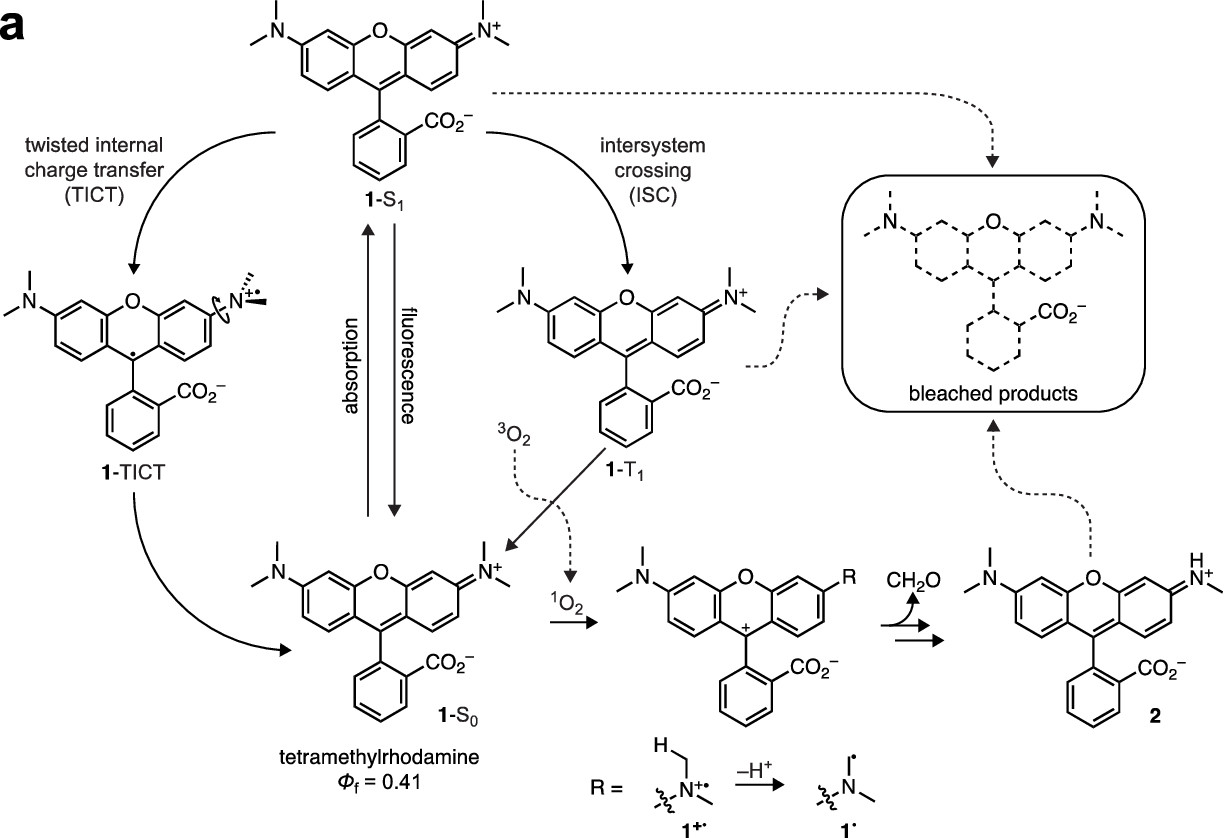
\includegraphics[width=10cm]{Rhodamines.png}
\end{figure}
\begin{itemize}
\item  Reduction of the T1 state yields a dark, long-lived, and stable radical state
\end{itemize}
\end{frame}

\begin{frame}{Dense labeling of histone H2B in fixed cells at RT}
\begin{textblock*}{11cm}(2.0cm,1.3cm)
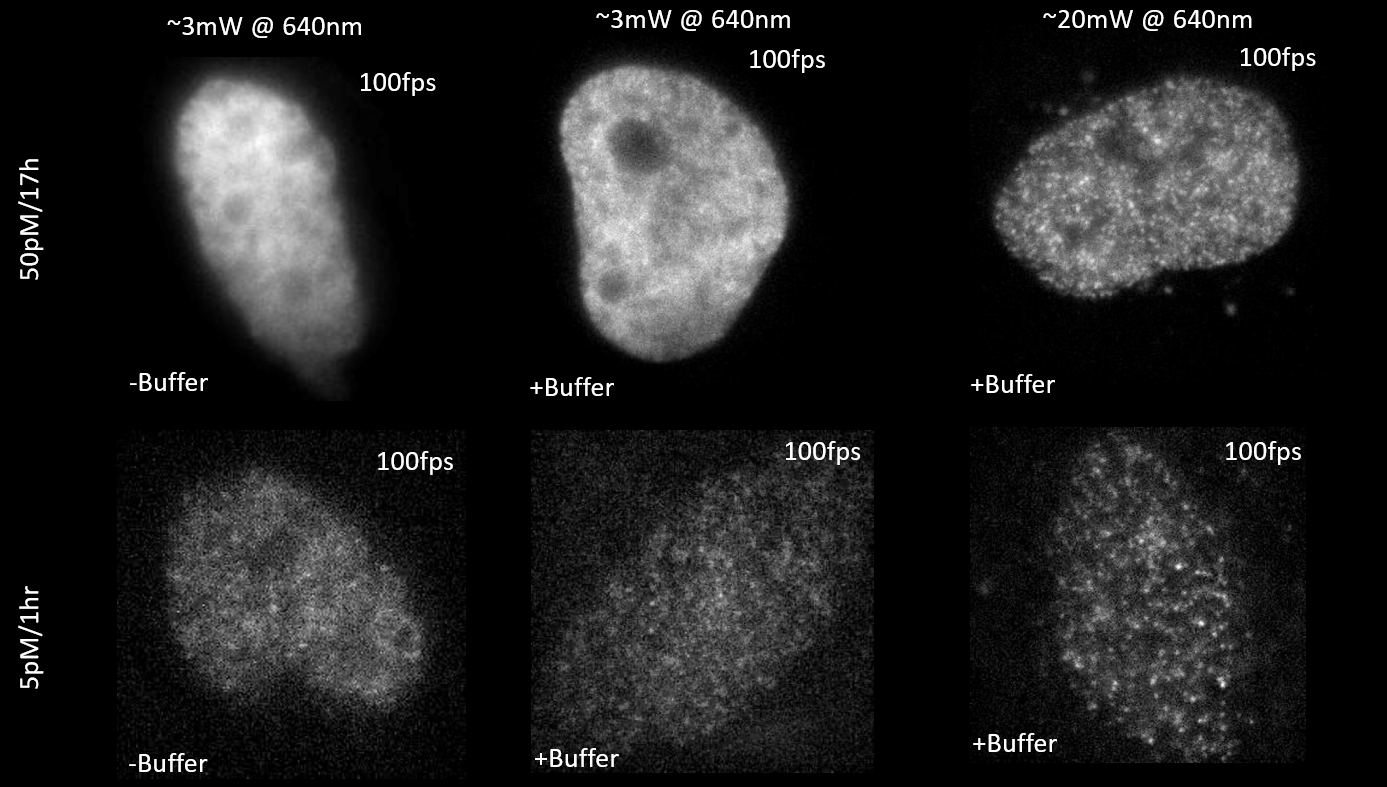
\includegraphics[width=11cm]{Laser.png}
\end{textblock*}
\begin{textblock*}{\textwidth}(0.5cm,8.0cm)
\begin{itemize}
\item Dense labeling of H2B-Halotag w/ fluorescent ligand JF646
\item Reducing buffer is usually a primary thiol like cysteamine (MEA)
\item Photoswitching of JF646 allows us to beat the diffraction limit
\end{itemize}
\end{textblock*}
\end{frame}

\begin{frame}
\frametitle{Direct stochastic optical reconstruction microscopy}

\begin{figure}
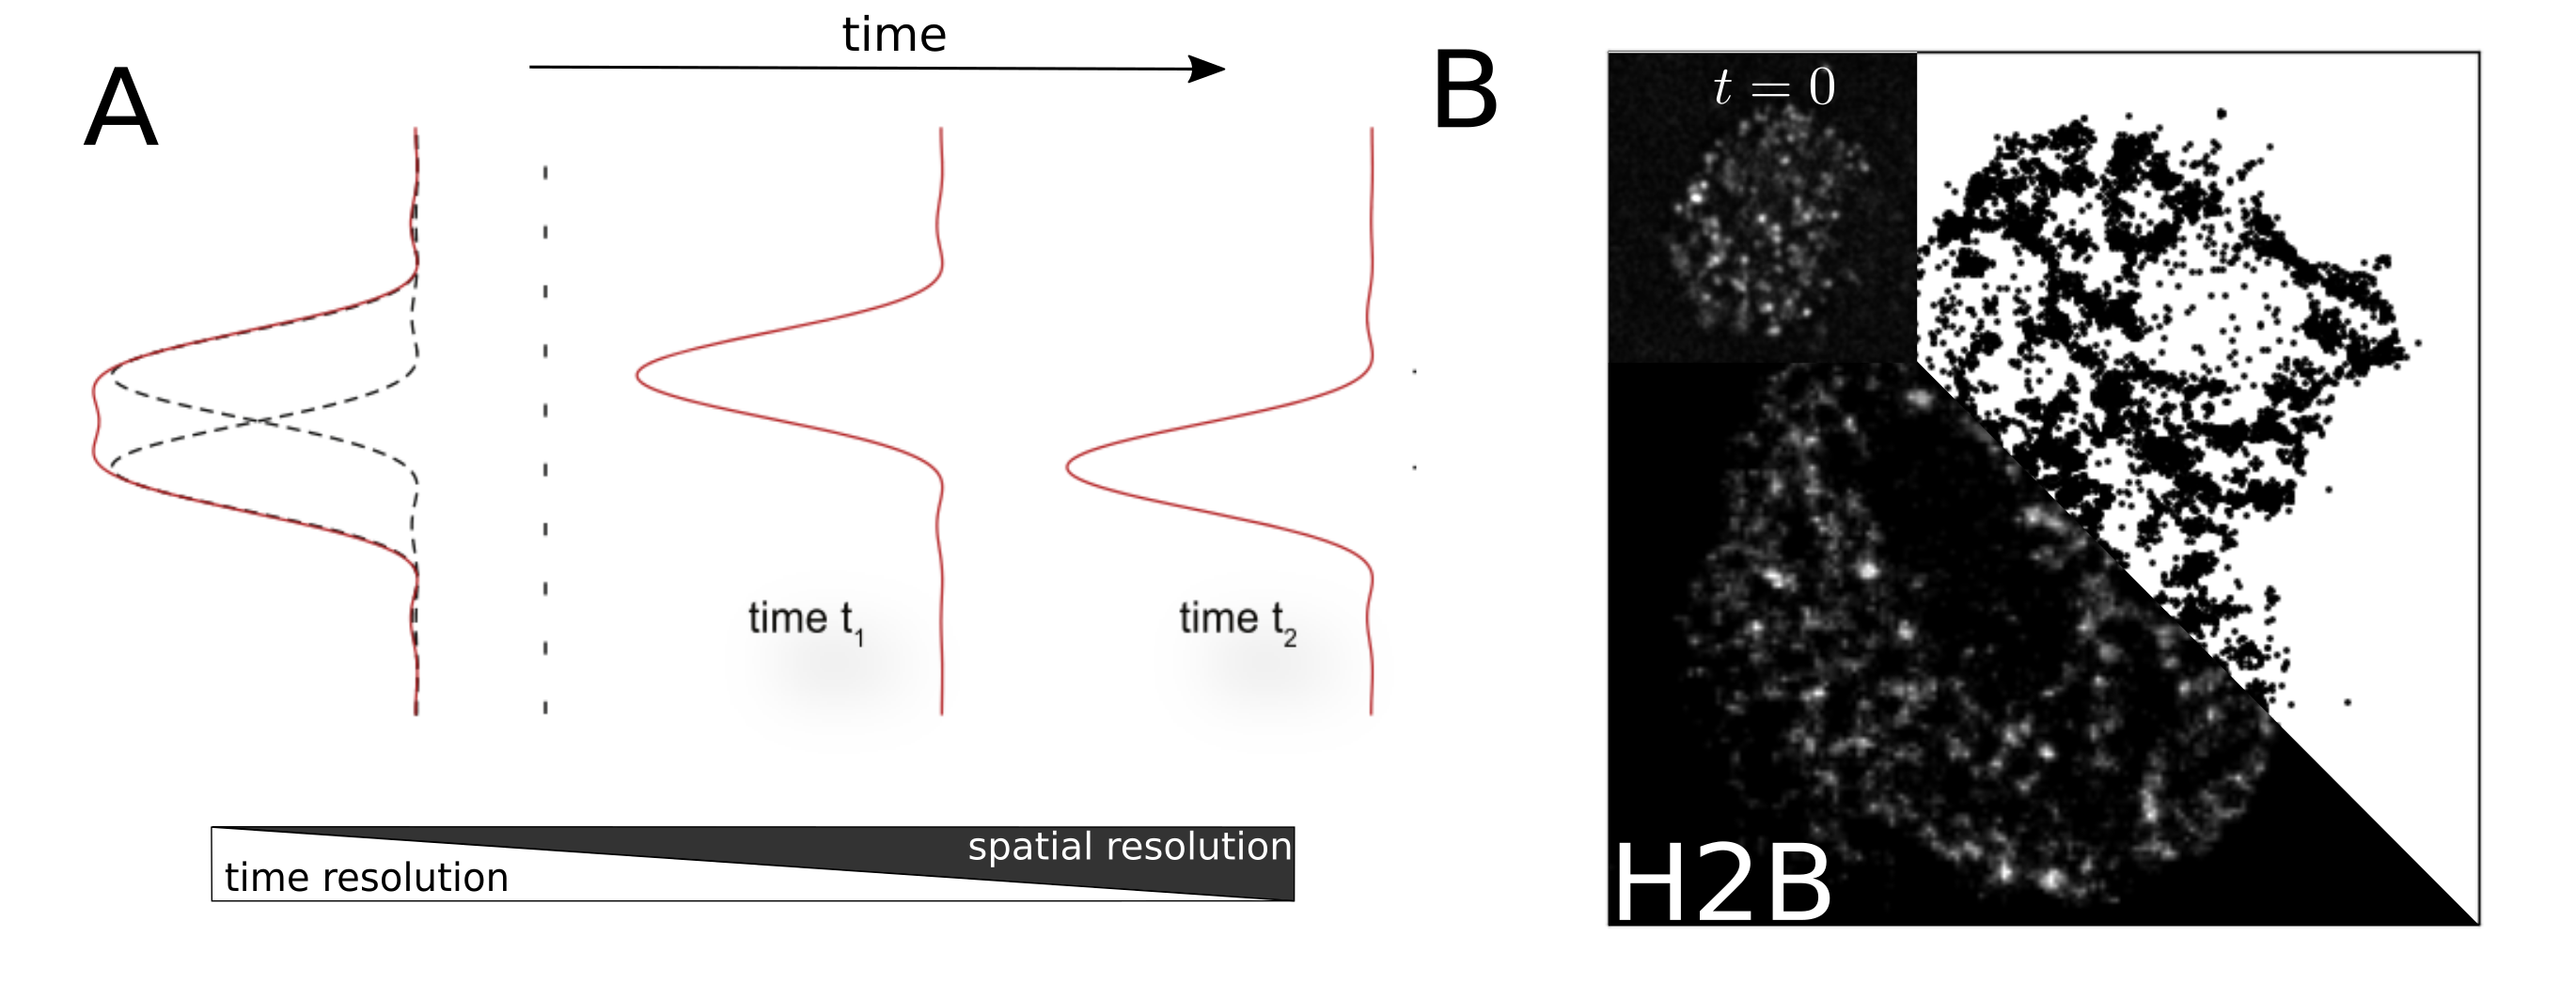
\includegraphics[width=13cm]{Concept.png}
\end{figure}

\begin{itemize}
\item Photoswitching enables resolution of emitters in time rather than space
\item Presents a tradeoff between spatial and temporal resolution
\end{itemize}

\end{frame}

\begin{comment}
\begin{frame}
\frametitle{Instrumentation for single molecule localization microscopy}

\begin{figure}
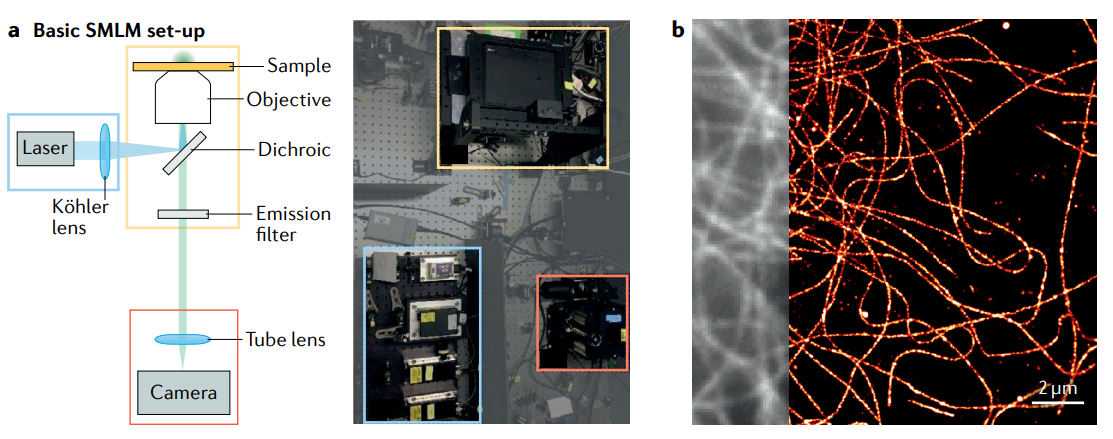
\includegraphics[width=12cm]{Setup.png}
\end{figure}

\begin{itemize}
\item Selectable widefield and oblique illumination
\item Widefield useful for high throughput 
\item Oblique method illuminates a thin section of nuclei
\end{itemize}

\end{frame}
\end{comment}


\section{The time resolution of \textit{d}STORM}
\begin{frame}{Fourier ring correlation links spatial and temporal resolution}
\begin{textblock*}{13cm}(1cm,1.25cm)
\begin{itemize}
\item We can view dSTORM as sampling from a density
\end{itemize}
\end{textblock*}
\begin{textblock*}{9cm}(3cm,2.0cm)
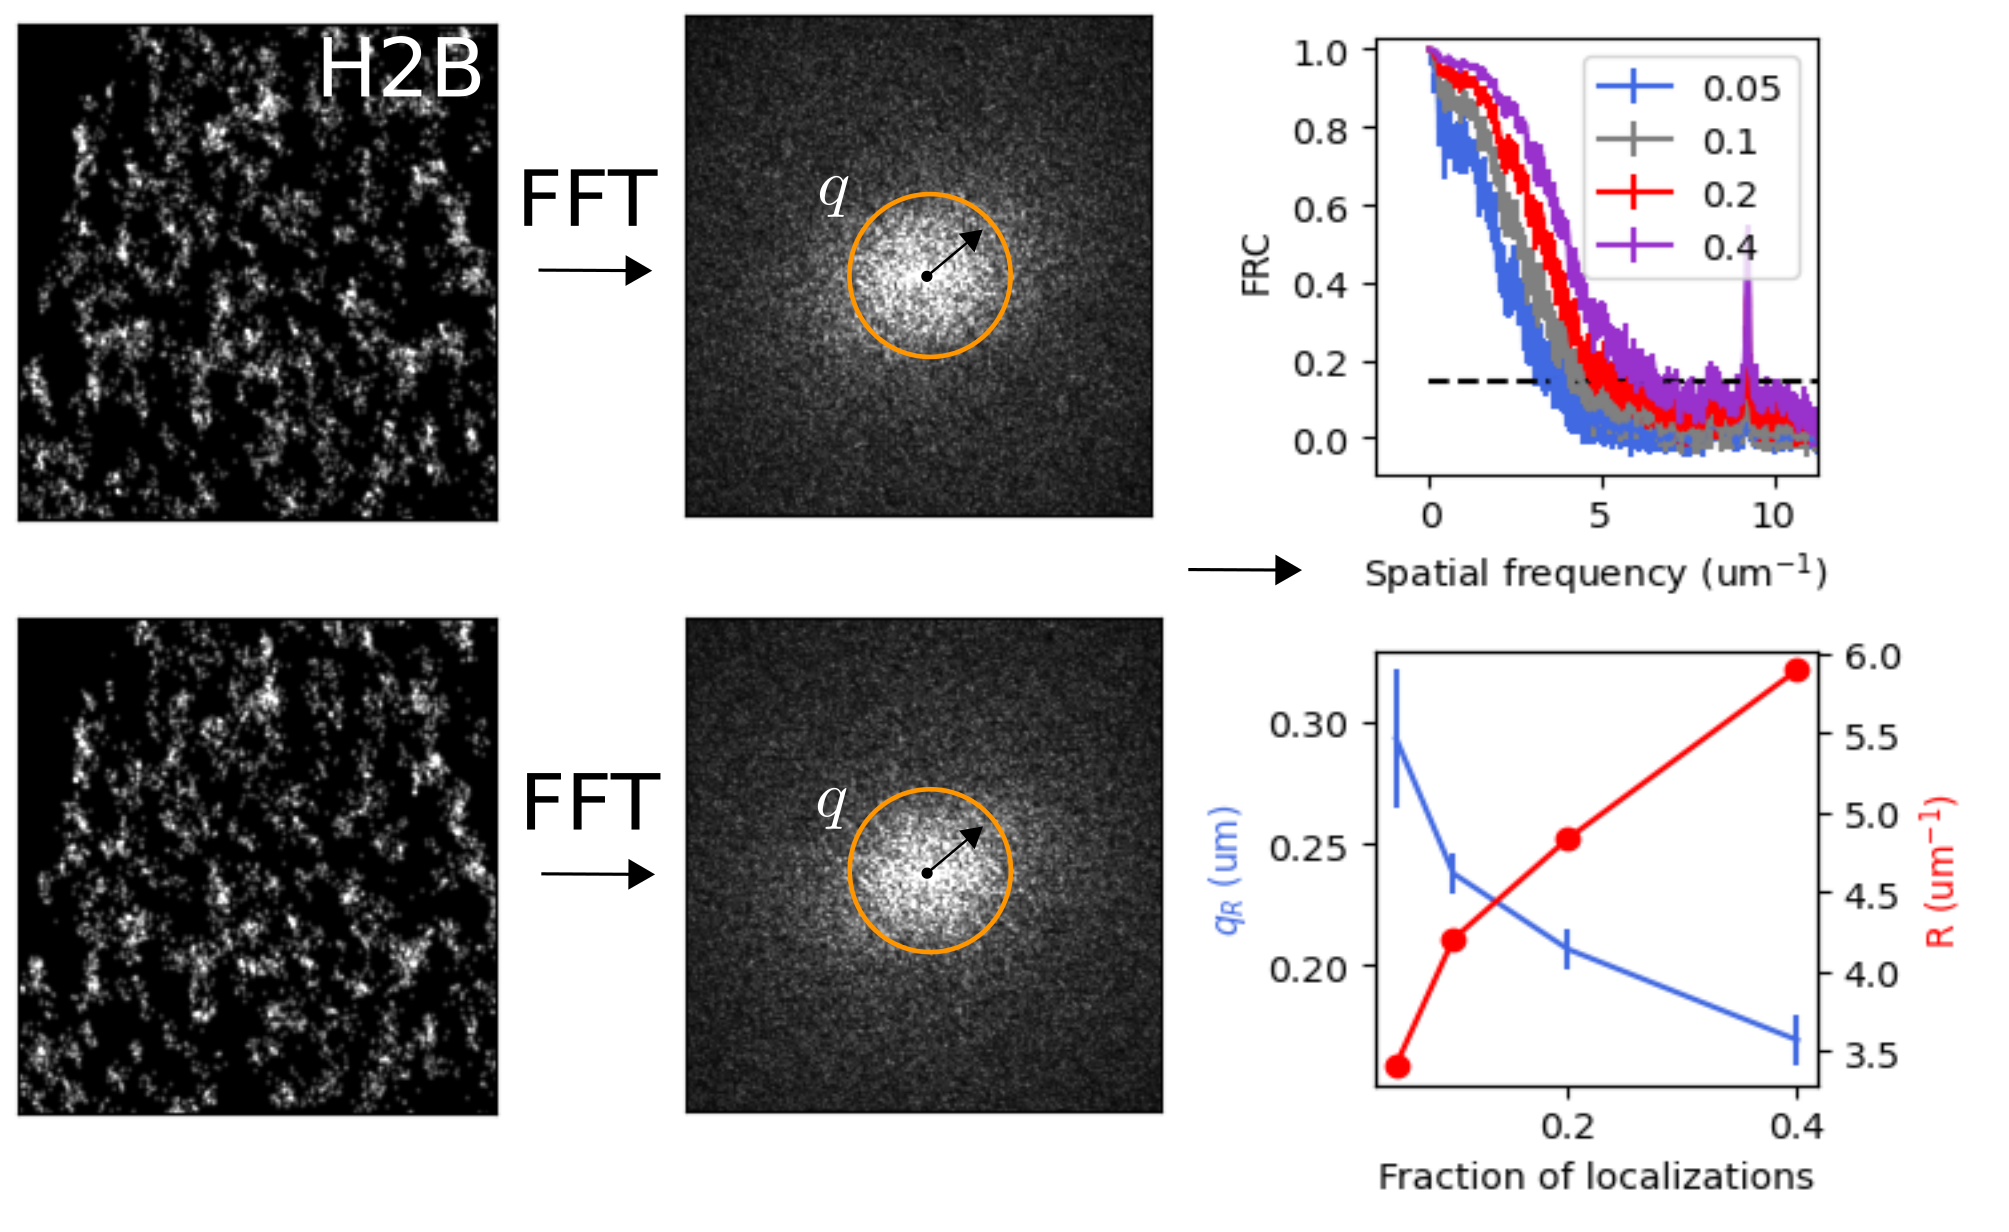
\includegraphics[width=9cm]{FRC.png}
\end{textblock*}
\begin{textblock*}{8cm}(3cm,7.5cm)
\begin{equation*}
\mathrm{FRC}(q) = \frac{\sum_{\vec{q}\in\mathrm{circle}}\tilde{f_{1}}(\vec{q})\tilde{f_{2}}(\vec{q})^{*}}{\sqrt{\sum_{\vec{q}\in\mathrm{circle}}|f_{1}(\vec{q})|^{2}}\sqrt{\sum_{\vec{q}\in\mathrm{circle}}|f_{2}}(\vec{q})|^{2}}
\end{equation*}
\end{textblock*}
\end{frame}

\begin{frame}{Fourier ring correlation links spatial and temporal resolution}
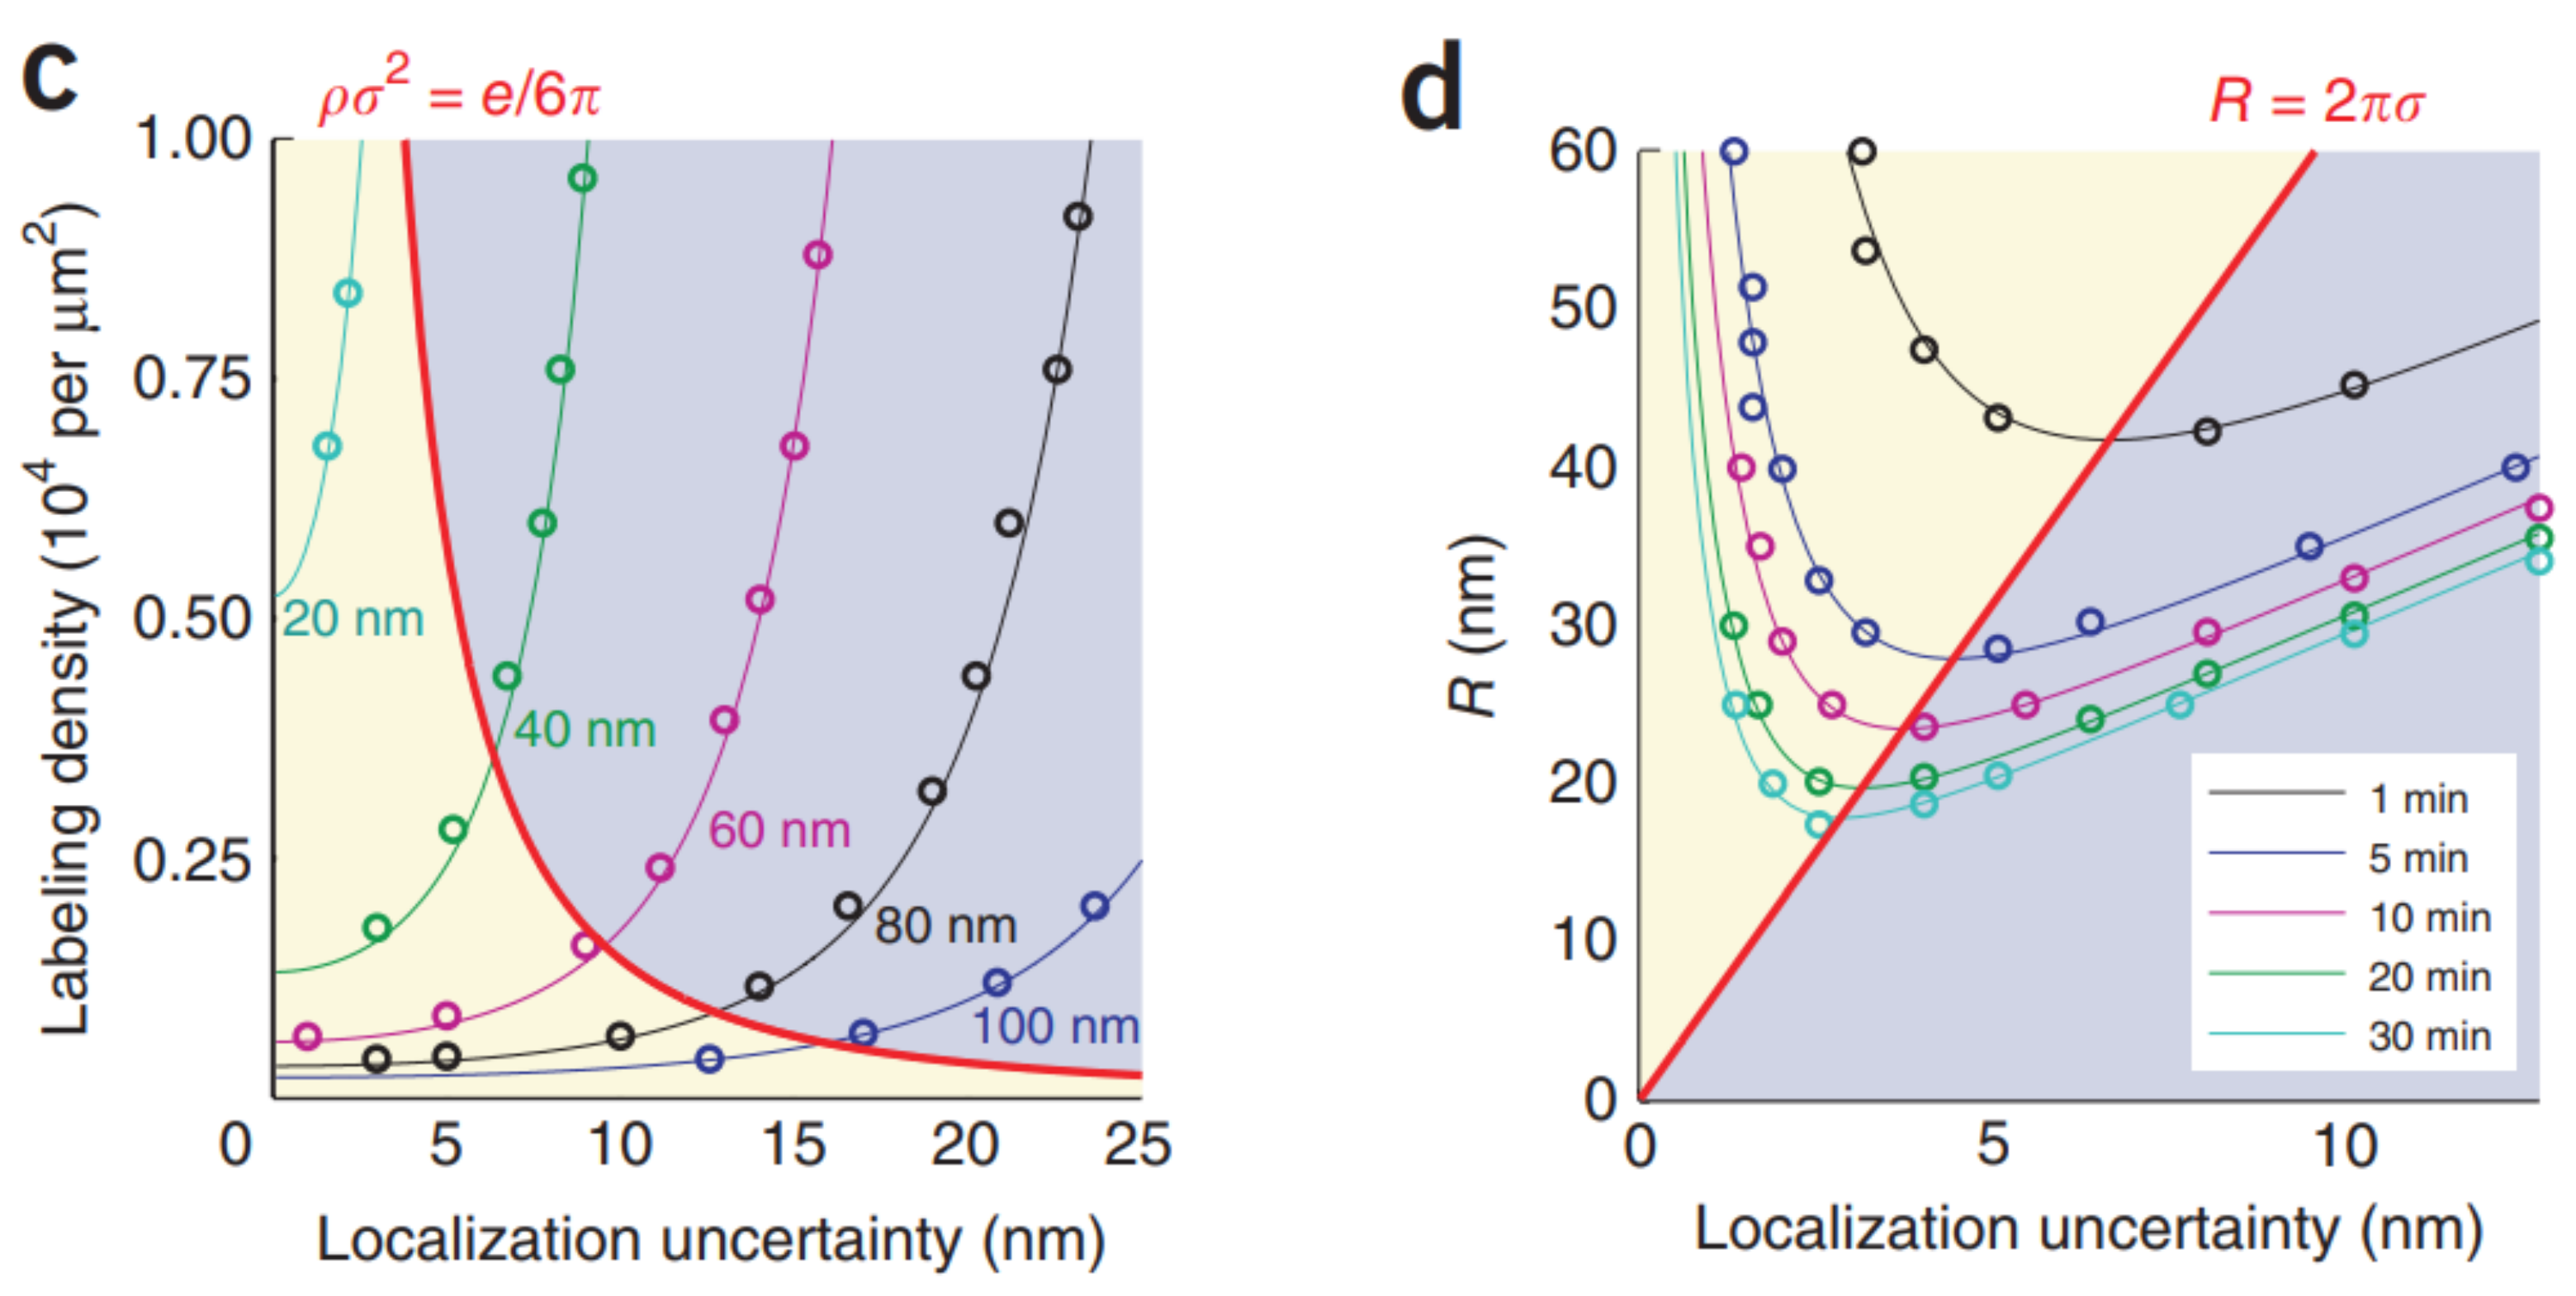
\includegraphics[width=\textwidth]{Spatial.png}
\textit{Nieuwenhuizen et al. Measuring image resolution in optical nanoscopy.}\\
\begin{itemize}
\item Increased localization uncertainty requires higher density for same resolution
\item Longer acquisitions have higher resolution
\end{itemize}

\end{frame}

\section{Dense localization with deep learning}

\begin{frame}{Estimator precision sets the resolution limit in localization microscopy}

\begin{textblock*}{10cm}(1.25cm,1.5cm)
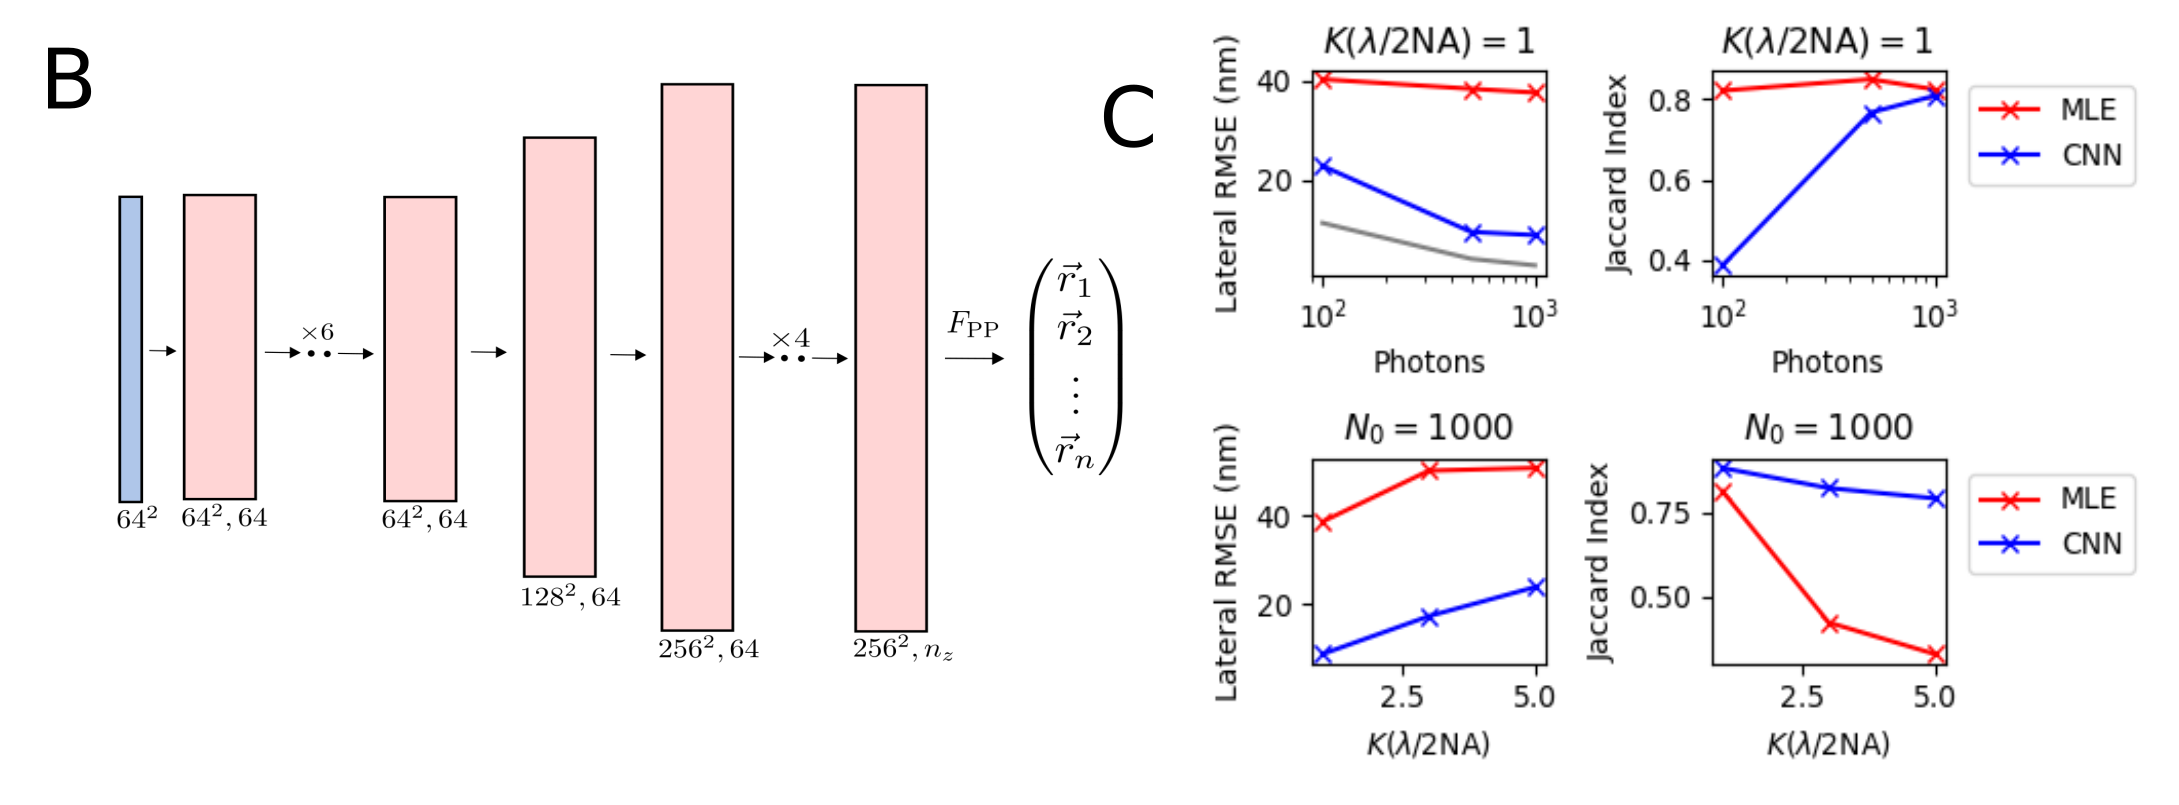
\includegraphics[width=13cm]{PSF2D-Crop.png}
\end{textblock*}
\begin{textblock*}{13cm}(1.25cm,7cm)
\begin{itemize}
\item $K(\lambda/2\mathrm{NA})$ is Ripley's K function at the diffraction limit ($\lambda=640\mathrm{nm}$)
\item Convolutional neural networks (CNNs) approach the Cramer-Rao lower bound (gray)
\end{itemize}
\end{textblock*}

\end{frame}

\begin{frame}{Chromatin nanodomains in a living Hela cell nucleus}

\begin{textblock*}{13cm}(0.5cm,1.5cm)
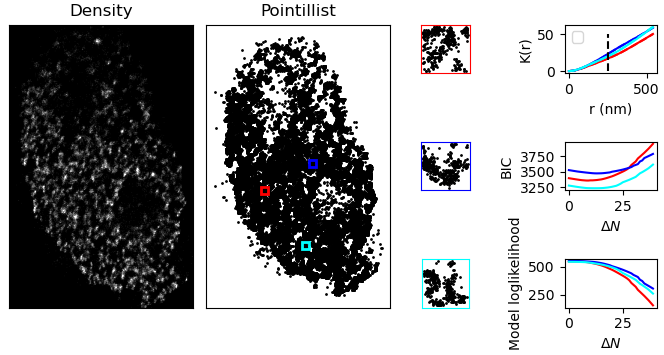
\includegraphics[width=\textwidth]{Cluster.png}
\end{textblock*}

\begin{textblock*}{13cm}(0.5cm,8.0cm)
\begin{itemize}
\item Histone DE using 30x30nm bins
\item Likelihood is computed under a Gaussian Mixture Model (GMM)
\end{itemize}
\end{textblock*}

\end{frame}

\section{Dense localization by fluorescence antibunching}

\begin{comment}
\begin{frame}{Next generation SMLM with photon counting cameras}

SOFI techniques conventionally compute autocorrelation functions $G_{ii}^{2}(\bm{r},\tau)$

SOFI images are usually $G^{2}_{ii}(\bm{r},0)$ for each pixel, for long integration times

It is reasonable that $G_{ij}^{2}(\bm{r}_{i},\bm{r}_{j},\tau)$ contains information about molecular positions

\begin{figure}
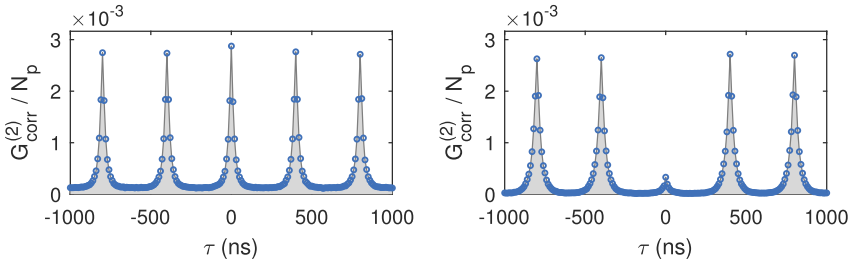
\includegraphics[width=10cm]{G2.png}
\end{figure}

For single photon counts, I don't think $G_{ij}^{2}(\bm{r}_{i},\bm{r}_{j},0)$  contains this information (peaks in $G_{ij}^{2}$ at nonzero lag is evidence for position)
Cross-cumulants may be more appropriate (Girsault 2016), which comes with virtual pixels
May also need pulsed excitation synced with the SPAD camera (can guarantee single photon per molecule per frame)
Higher order correlations might give stronger localization results, but could be intractable to compute (RNNs?)

\end{frame}

\end{comment}

\begin{comment}
\begin{frame}
Now I'm not so sure that the shape of $G_{ij}^{2}$ contains information on position. Translating a molecule along the axes changes the intensity of the individual processes, and I don't believe $G_{ij}^{2}$ is sensitive to the intensity of the processes.
Imagine a molecule emits $N$ photons. As the molecule approaches the neighboring pixel, more photons hit the neighboring pixel, but the delay between consecutive photons hitting pixel 2 and pixel 1 is unchanged. 

However, the intensity information and the anticorrelation of the processes are complementary. The degree of anticorrelated-ness of the various pairs determines how we can "group the pixels". Intensities then could then be used in a full generative model for the data.

A molecule at position $\theta$ will result in anticorrelated neighboring pixels. Perhaps $G_{ij}^{2}(\bm{r}_{i},\bm{r}_{j},0)$ can be use to determine how anti-correlated the pixels are. Then, we use this value to create the "virtual pixels". Then define a likelihood function on the pixels+virtual pixels given the coordinates. 

\end{frame}
\end{comment}

\begin{comment}
\begin{frame}{Dense localization by fluorescence antibunching}

If the emission from a single molecule represents a sub-Poisson process, then the detection process is also sub-Poisson, with a reduced rate. 

Consider point processes $n_{i}(t)$ and $n_{j}(t)$. The second order coherence function reads

\begin{equation*}
g^{2}_{ij}(\tau) = \frac{\langle n_{i}(t+\tau)n_{j}(t)\rangle}{\langle n_{i}(t)\rangle\langle n_{j}(t)\rangle}
\end{equation*}

$n_{i}(t)$ and $n_{j}(t)$ are parameterized by $\theta$. Suppose they are Poisson processes, with rates that can be computed from $\theta$ e.g., $\mu_{i} = f(\theta)$ and $\mu_{j} = g(\theta)$. Then, 

\begin{equation*}
g^{2}_{ij}(0) = \frac{\langle n_{i}(t)n_{j}(t)\rangle}{\mu_{i}\mu_{j}} = 1
\end{equation*}

However, when they are sub-Poisson processes, then $\langle n_{i}(t)n_{j}(t)\rangle \leq \langle n_{i}(t)\rangle\langle n_{j}(t)\rangle$. Why?

The presence of multiple emitters in the local region makes photons appear more ``bunched" w.r.t these two detector elements $i$ and $j$, and therefore $g^{2}_{ij}(0) > 0$. I expect we can use $g^{2}_{ij}(0)$ over 3x3 neighborhoods of pixels where $i$ the center pixel.

\end{frame}
\end{comment}

\begin{comment}
\begin{frame}{Dense localization with fluorescence antibunching}

We require an estimate of emitter locations $\theta^{*}$ to approximate 

\begin{itemize}
\item The number of photons collected in each pixel \\
\item The second order coherence of photon counts in a pixel with its neighbors 
\end{itemize}

Defining a likelihood on the entire time series is intractable. In intensity-based imaging, we would just analyze the sum of photon counts over time. However, the number of emitters is unknown \emph{a priori}, which is part of the problem we are trying to solve. Instead we approximate the maximum likelihood estimate by a stochastic \emph{online parameter estimation} procedure. I imagine emitters are added, if there is not reasonable probability that a photon was emitted by an existing one.

We are able to compute the likelihood of the time summed data and pairwise coherence calculations as the time series and optimization proceed.

\end{frame}
\end{comment}

\begin{frame}{Dense localization with fluorescence antibunching}

Suppose pixel $i$ collects $N_{i}$ photons and pixel $j$ collects $N_{j}$ photons. Index pair $(i,j)$ by $k$. Since pixels are independent

\begin{align*}
P(X_{i}=N_{i},X_{j}=N_{j}) &=P(X_{i}=N_{i})P(X_{j}=N_{j})\\
&=  \left[\sum_{\alpha}\left(\prod_{n}p_{i}^{\alpha_{n}}(1-p_{i})^{1-\alpha_{n}})\right)\right]\left[\sum_{\beta}\left(\prod_{n}p_{i}^{\beta_{n}}(1-p_{i})^{1-\beta_{n}})\right)\right]
\end{align*}

where $\alpha,\beta$ are binary strings indicating which emitters contribute to the count. $\Omega_{k}$ has the dimension of the state space of $(X_{i},X_{j})$. Clearly,$\sum_{n}\alpha_{n} = N_{i}$ and $\sum_{n}\beta_{n} = N_{j}$. Also, due to independence

\begin{equation*}
\langle X_{i}X_{j} \rangle = \langle X_{i}\rangle\langle X_{j} \rangle 
\end{equation*}

\end{frame}


\begin{frame}{Dense localization by fluorescence antibunching}
\begin{textblock*}{12cm}(1.5cm,1.0cm)
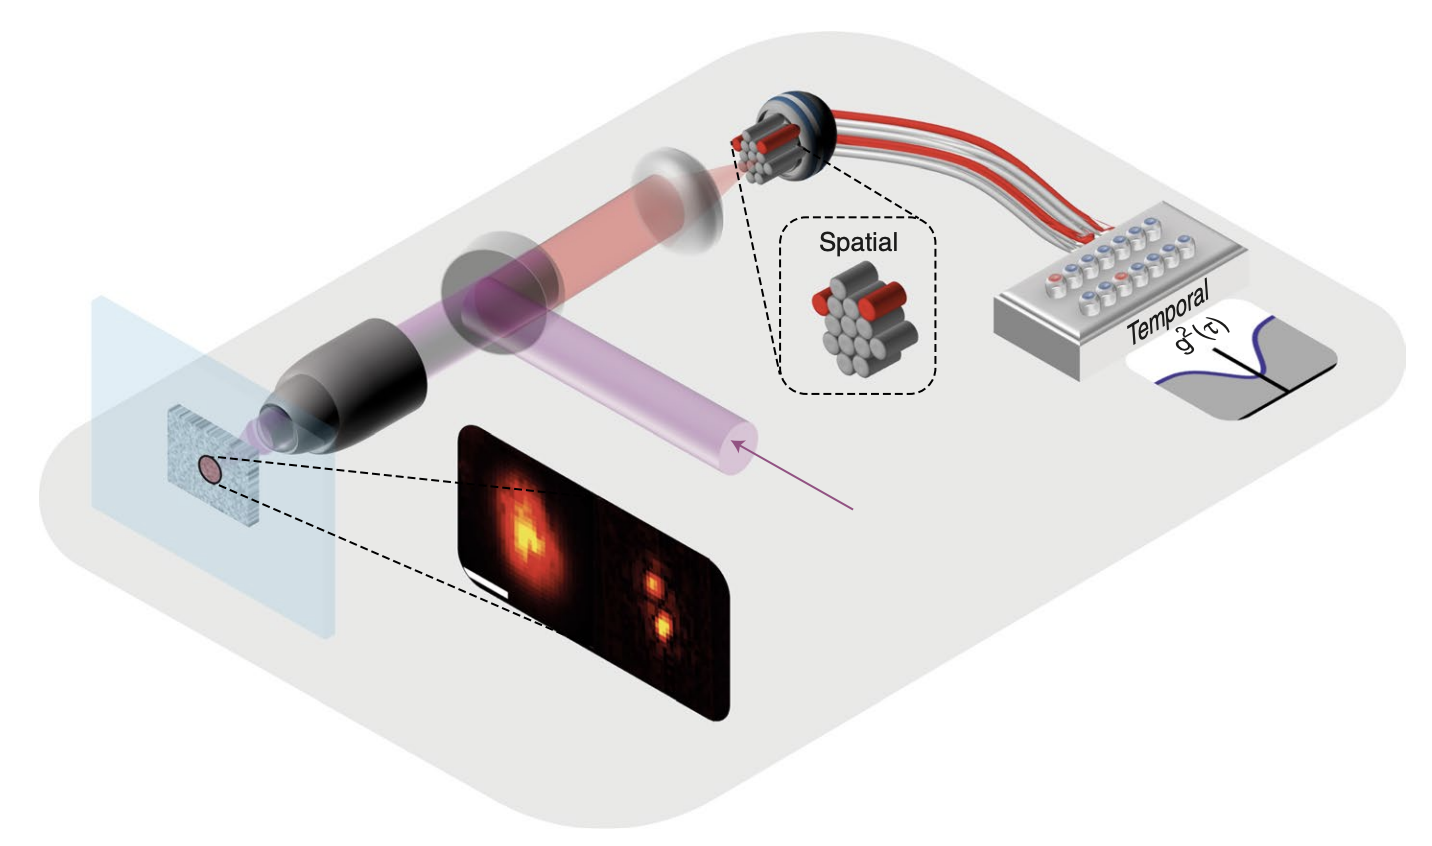
\includegraphics[width=12cm]{Quantum.png}
\textit{Andrew Forbes and Valeria Rodriguez-Fajardo. Super-resolution with quantum light. Nature Photonics 2019.}
\end{textblock*}
\end{frame}

\begin{comment}
\begin{frame}{Chemical fixation changes the appearance of nucleosome clustering}
\begin{textblock*}{12cm}(1.5cm,1.75cm)
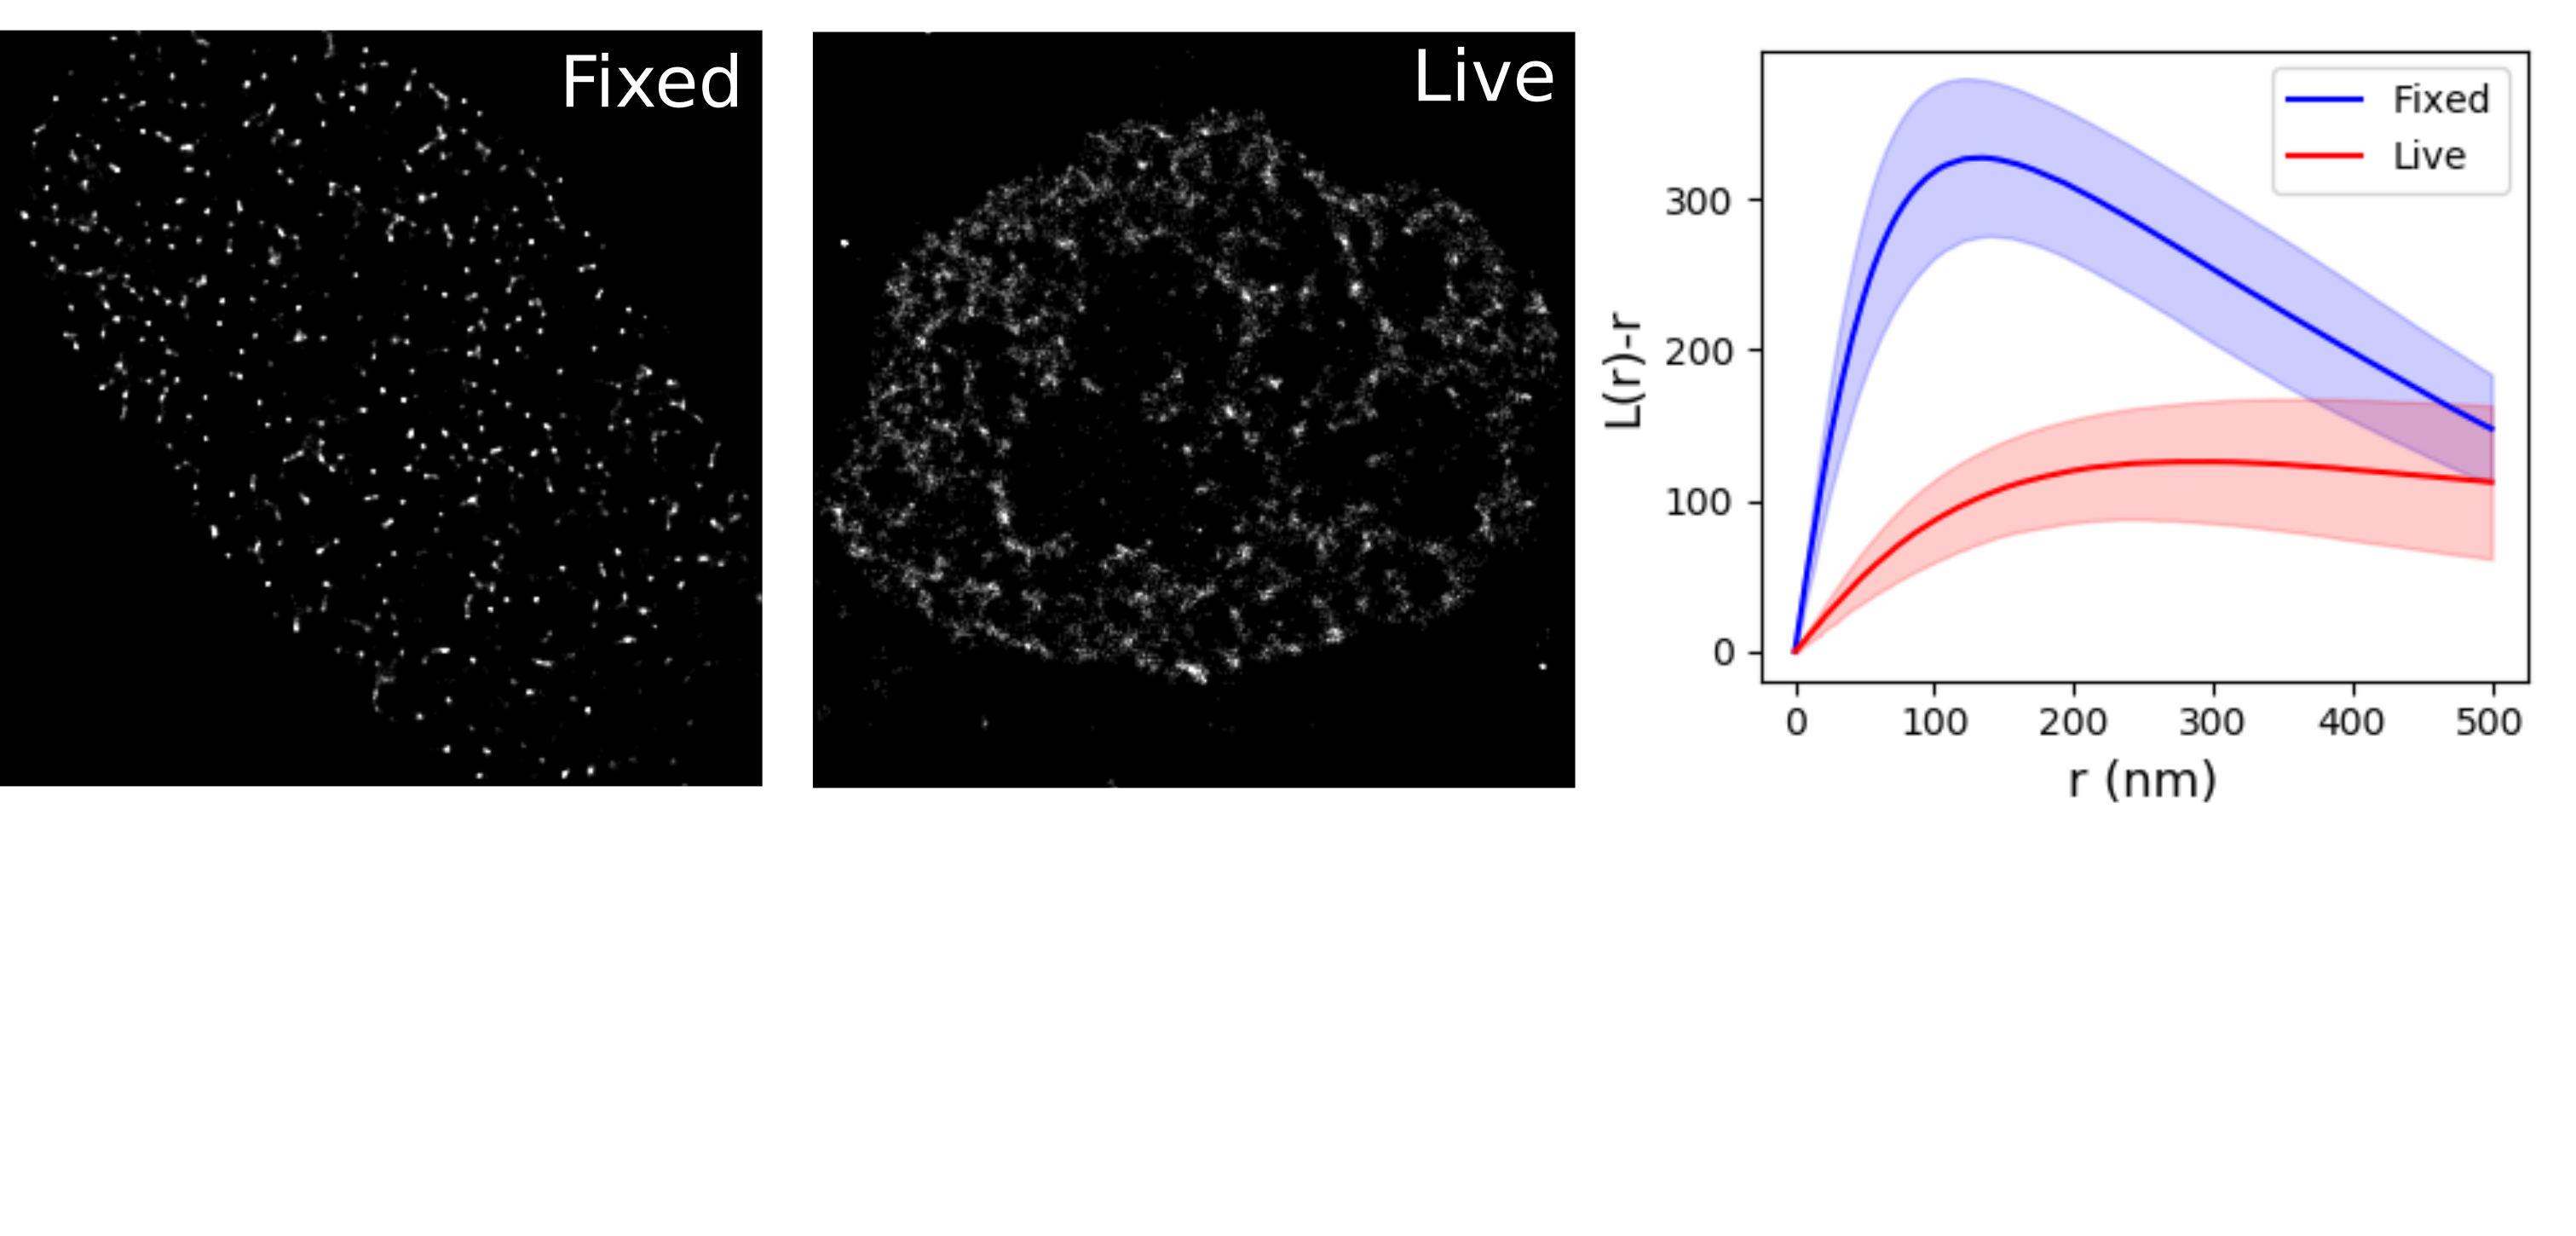
\includegraphics[width=\textwidth]{LiveFix.png}
\end{textblock*}
\end{frame}
\end{comment}

\begin{frame}{Inhibition of a super-enhanced gene with JQ1}
\begin{figure}
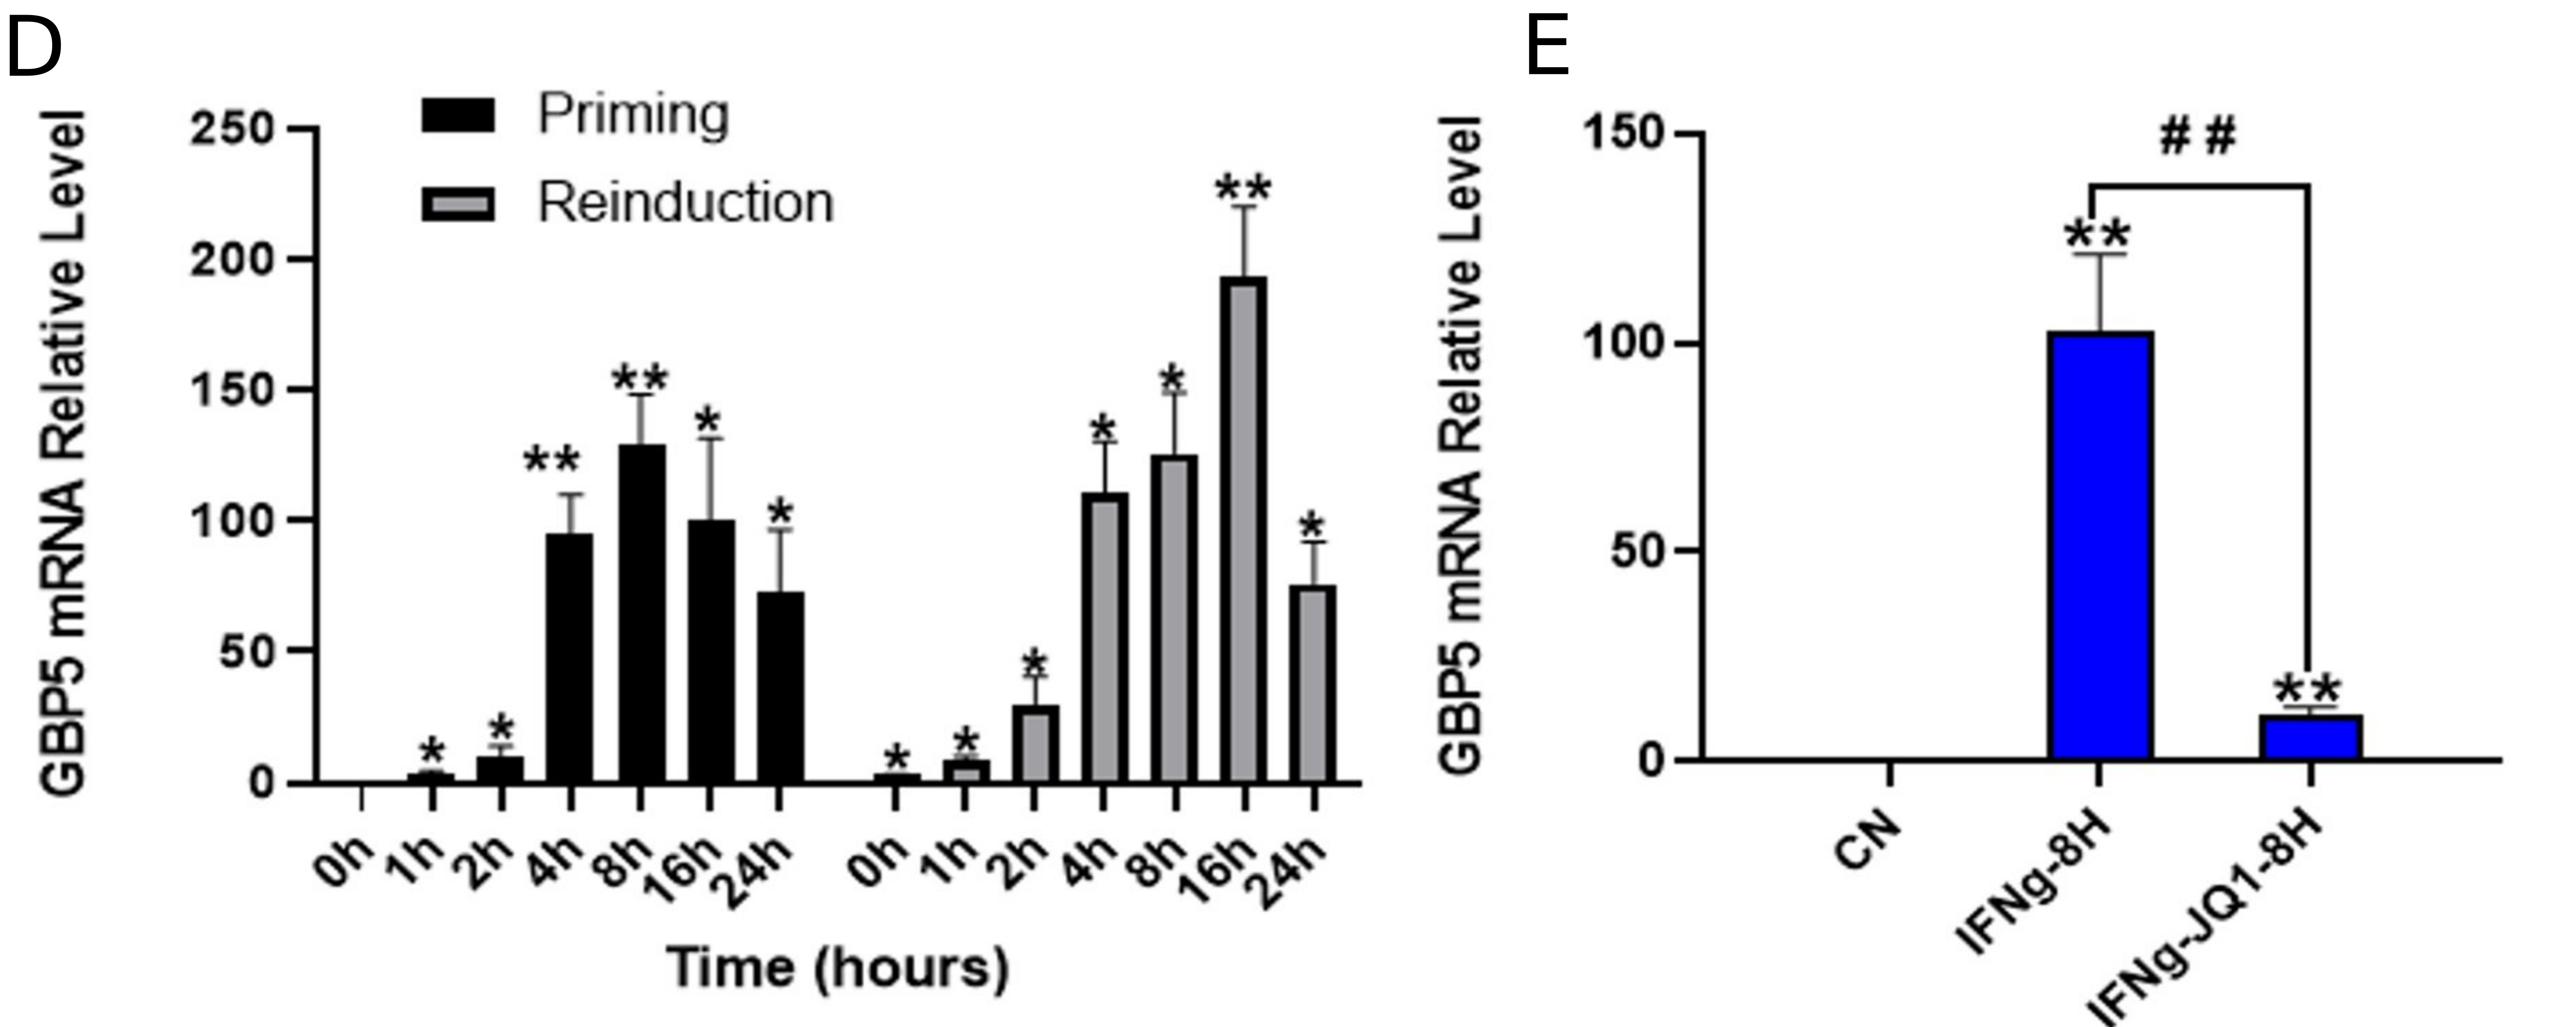
\includegraphics[width=12cm]{GBP5-2.png}
\end{figure}
\begin{itemize}
\item *:$P \leq 0.1$, **:$P \leq 0.01$
\end{itemize}
\end{frame}

\section{The nucleosome: lost in phase space}

\begin{comment}
\begin{frame}{Astigmatism based three dimensional imaging}
\begin{figure}
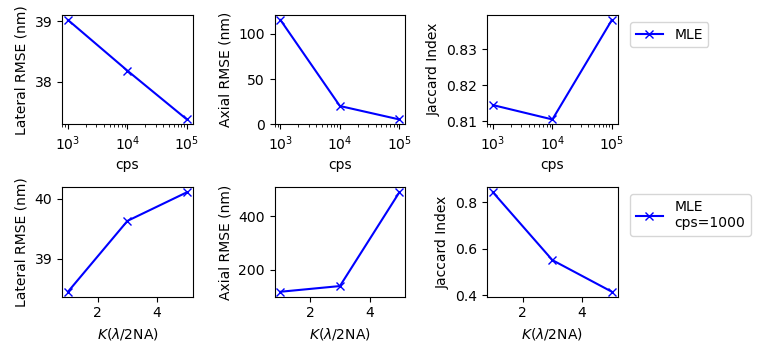
\includegraphics[width=13cm]{PSF3D.png}
\end{figure}
\begin{itemize}
\item $z_{0}\sim U([-0.4,0.4])$ um
\item 3D imaging requires long exposure and sparse emitters for MLE
\item Deep methods may be a suitable choice in future work
\end{itemize}
\end{frame}
\end{comment}

\begin{comment}
\begin{frame}{Astigmatism based three dimensional imaging}
\begin{figure}
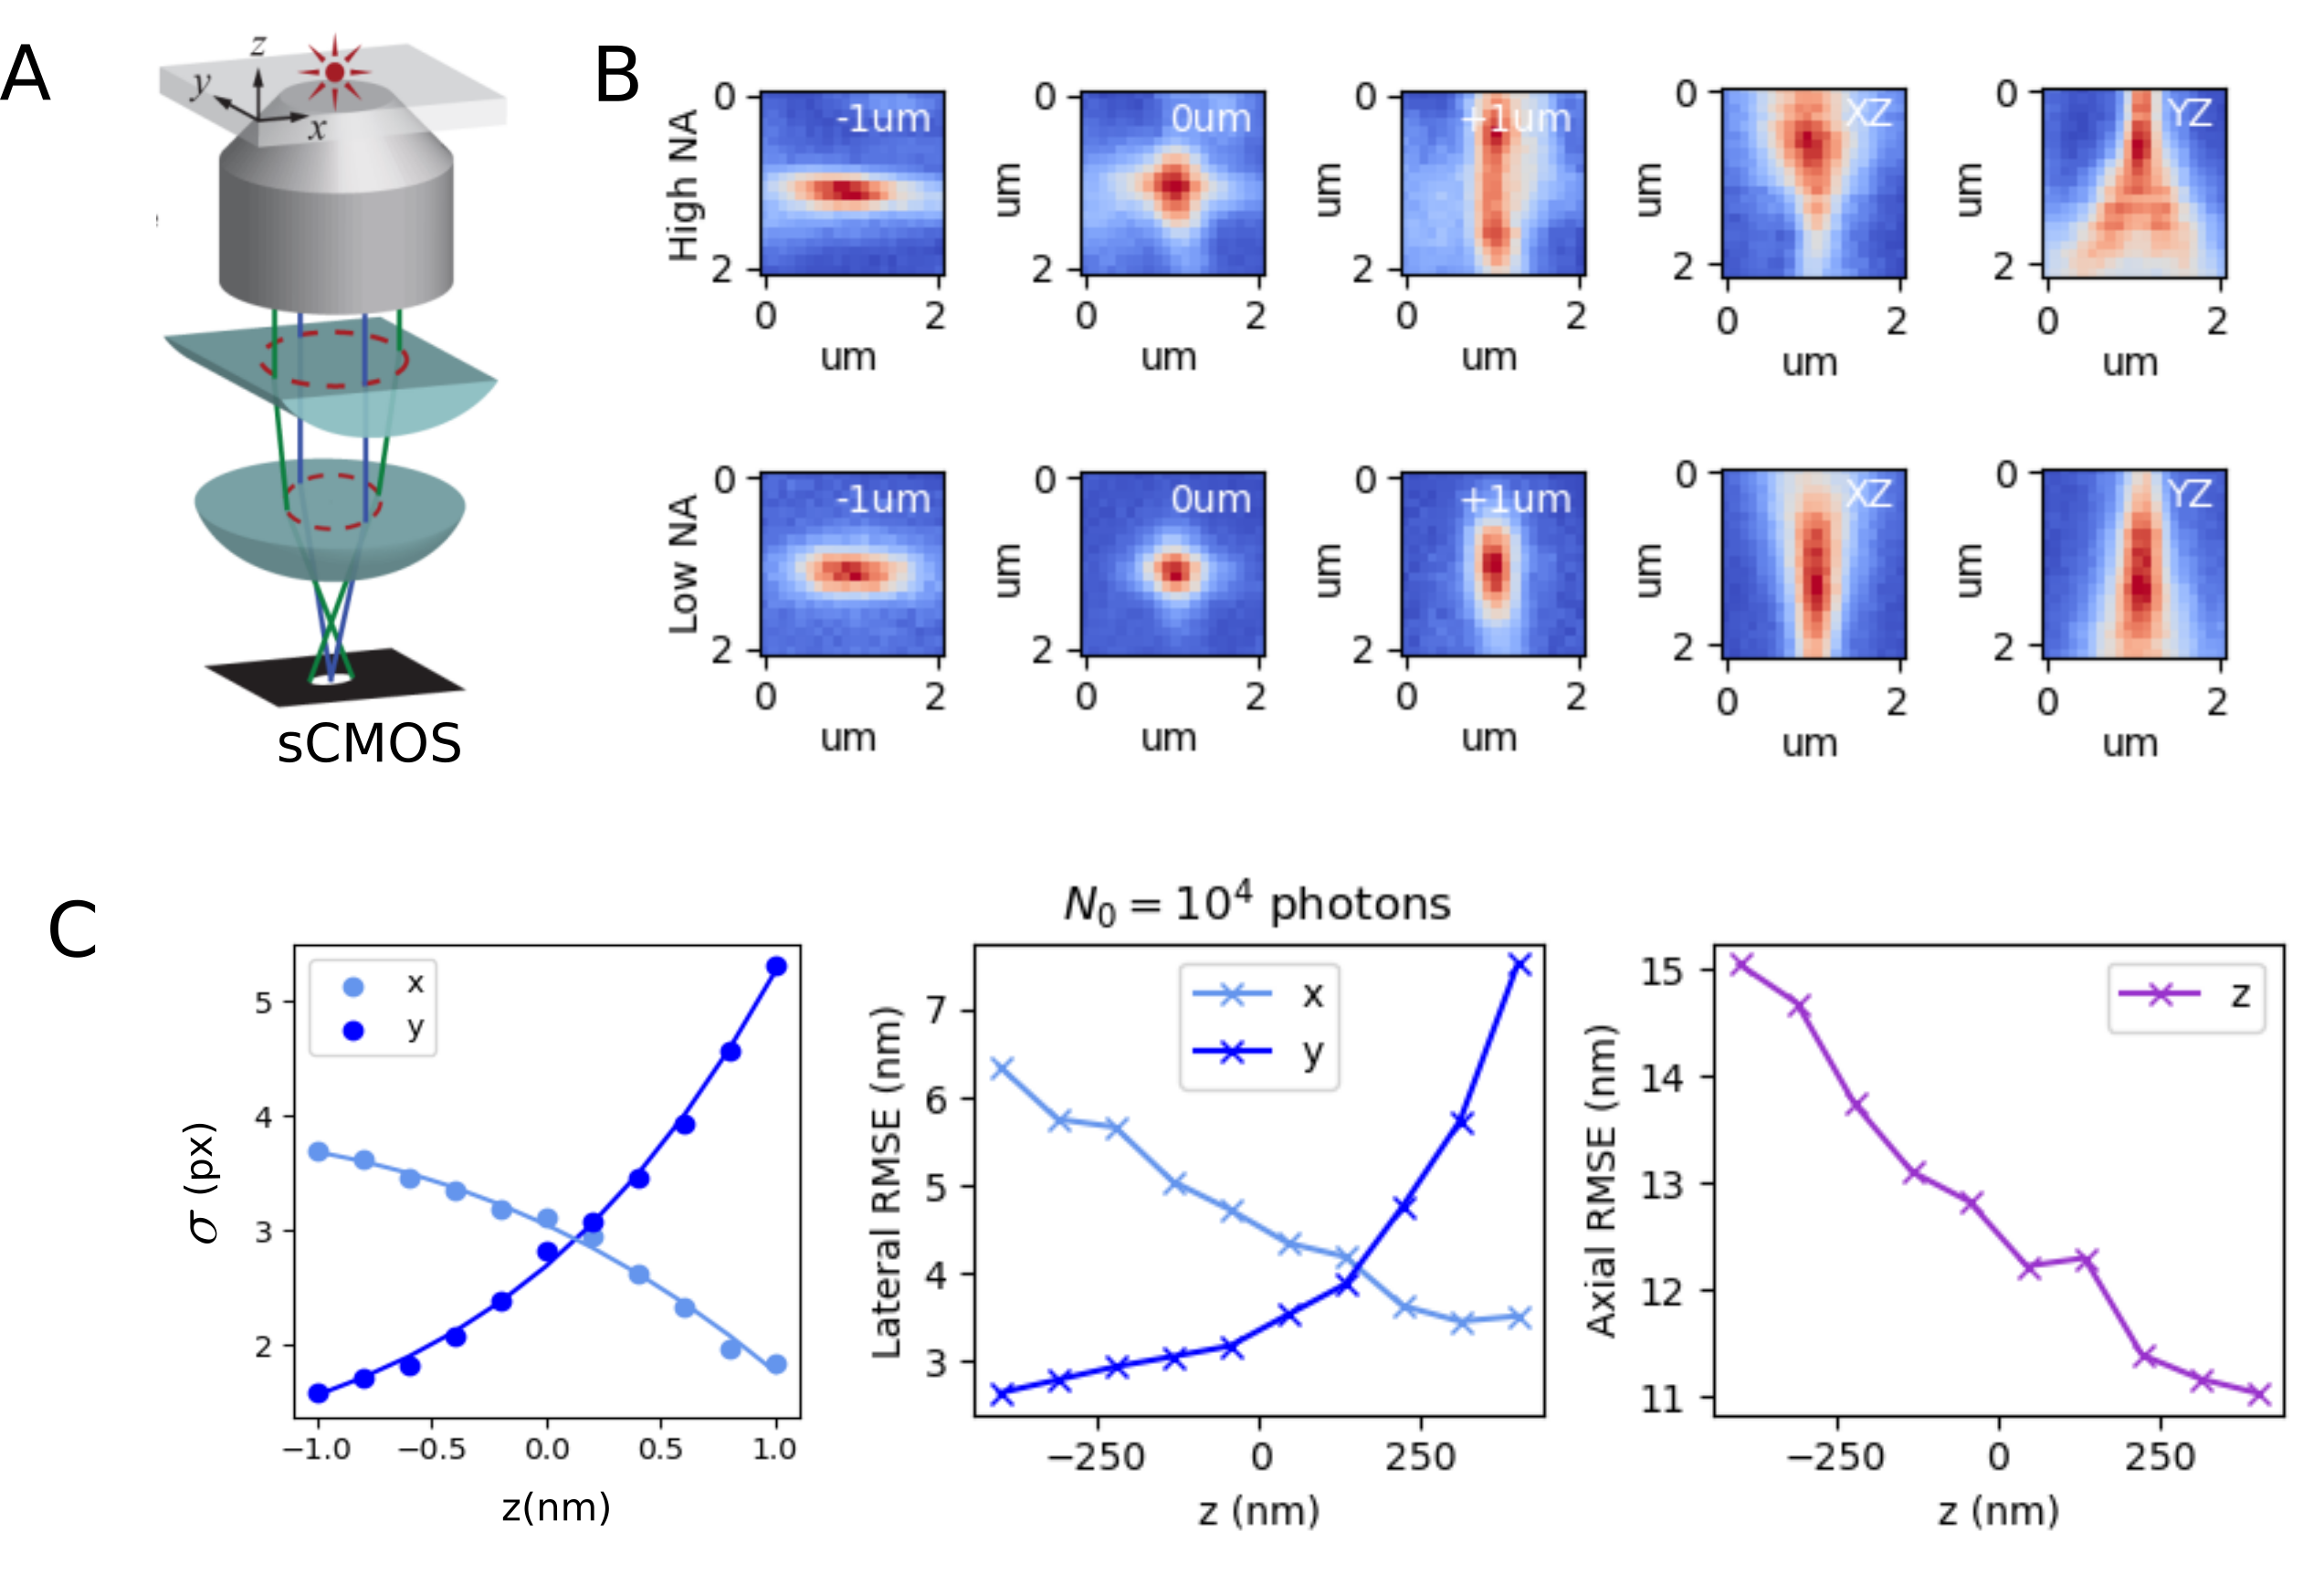
\includegraphics[width=11cm]{Astigmatism.png}
\end{figure}
\begin{itemize}
\item A weak ($f=10$m) cylindrical lens breaks the axial symmetry of the PSF
\end{itemize}
\end{frame}
\end{comment}


\section{Phase separation of chromatin}
\begin{frame}{Chromatin has an intrinsic ability to undergo phase separation}

\begin{textblock*}{10cm}(2.25cm,1.5cm)
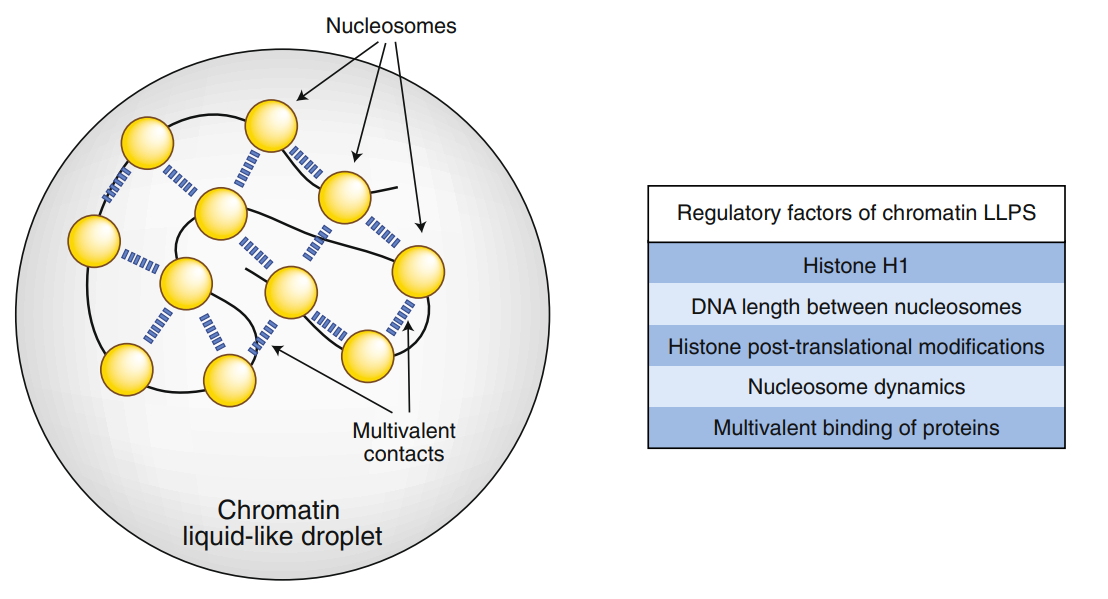
\includegraphics[width=10cm]{ChromatinLLPS.png}
\end{textblock*}


\begin{textblock*}{14cm}(0.5cm,7.5cm)
\begin{itemize}
\item Super-enhanced genes are regulated by large molecular assemblies
\item We study nucleosome clustering dynamics using super-resolution microscopy
\end{itemize}
\end{textblock*}

\end{frame}


\begin{frame}{(+)-JQ1 in complex with BRD4 protein}

\begin{textblock*}{6cm}(1.0cm,1.5cm)
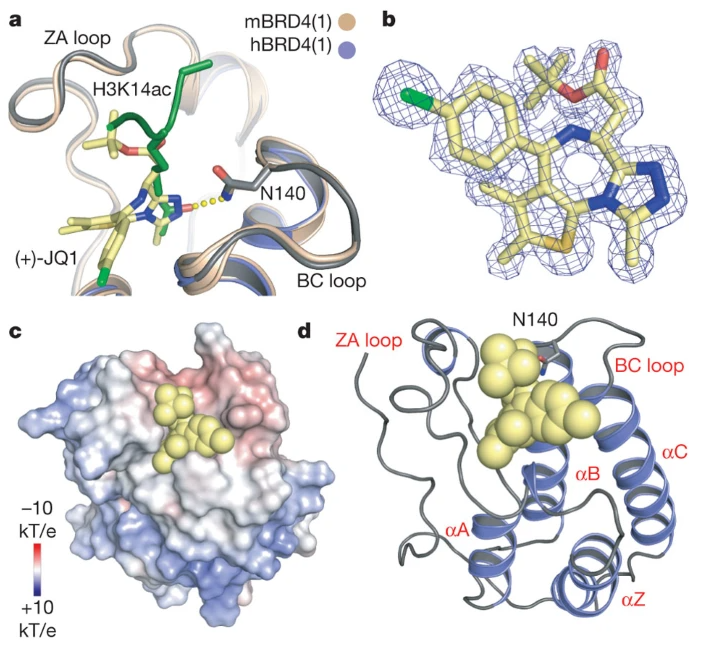
\includegraphics[width=6cm]{JQ1_Complex.png}
\end{textblock*}

\begin{textblock*}{8cm}(7.5cm,1.75cm)
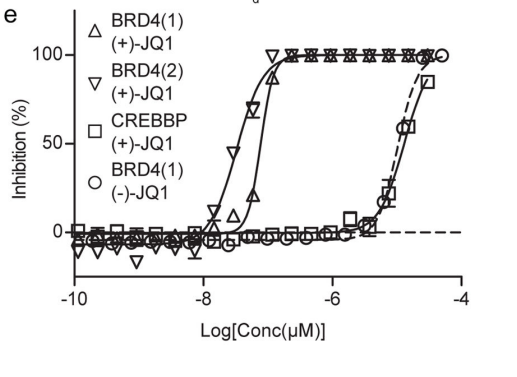
\includegraphics[width=8cm]{BRD4-Inhibition.png}
\end{textblock*}

\begin{textblock*}{\textwidth}(1.0cm,7.5cm)
\textit{Filippakopoulos. Selective inhibition of BET bromodomains. Nature }

\begin{textblock*}{14cm}(0.5cm,8.1cm)
\begin{itemize}
\item BRD4 is an interesting target since specific and non-specific inhibitors exist
\item BET mimics including +JQ1 prevent binding of BRD4 to acetylated histones
\end{itemize}
\end{textblock*}

\end{textblock*}

\end{frame}

\begin{frame}{BET inhibitors reduce nucleosome-BRD4 interactions in BRD4 condensates}
\end{frame}

\begin{frame}{BET inhibitors promote disordered BRD4 condensates }
\end{frame}



\begin{comment}
\begin{frame}{Inhibition of a super-enhanced gene with JQ1}
\begin{figure}
\includegraphics[width=13cm]{GBP5-1.png}
\end{figure}
Blue - DAPI (binds DNA minor groove)
\begin{itemize}
\item Guanylate binding proteins (GBPs) are a family of GTPases induced by IFN-$\gamma$
\item BRD4 is directly involved in GBP gene expression
\end{itemize}
\end{frame}
\end{comment}


\end{document}